\documentclass[10pt, a4paper]{report}
\usepackage[utf8]{inputenc}
\usepackage[T1]{fontenc}
\usepackage[english]{babel}
\usepackage{graphicx}
\usepackage{hyperref}
\usepackage[hypcap]{caption}

\begin{document}
\title{Pending}
\author{Alexandre Carlessi \and Sahand Kashani-Akhavan}
\date{\today}
\maketitle

\section*{Introduction}
A graphics processing unit, also known as a GPU, is a specialized electronic
circuit initially designed for fast memory manipulations needed to accelerate
the creation of images in a frame buffer, which are then outputted to a display
for viewing.
Nowadays, GPUs are present in almost all electronics, including, but not limited
to embedded systems, mobile phones, personal computers, workstations, and game
consoles.

Modern GPUs have highly parallel structures, making them much more effective
than general-purpose CPUs for algorithms which process large blocks of data in
parallel.
Thus, GPUs have become very efficient at manipulating imagery, which consists
of applying an algorithm parallely to all output pixels, which explains their
abundant use in computer graphics.

In this report, we look at ways to apply

\section*{Programmability}
GPUs were initially designed to accelerate texture mapping, polygon rendering,
and geometry.
The first GPUs had a fixed-function rendering pipeline, and could not be used
for anything other than common geometry transformations and pixel-shading
functions that were pre-defined in hardware.

With the introduction of the NVIDA GeForce 3 in 2001, GPUs added programmable
shading to their capabilities, which allowed developers to define their own
straight-line shading programs to perform custom effects on the GPU.
Bypassing the fixed-function rendering pipeline opened the door towards many
future graphics novelties, such as cel shading, mip mapping, shadow volumes,
oversampling, interpolation, bump mapping, and many others.

The 2 main shaders were the fragment shader (also known under the name of pixel
shader), and the vertex shader (also known under then name of geometry shader).
The vertex shader processed each geometric vertex of a scene and could
manipulate their position and texture coordinates, but could not create any new
vertices.
The vertex shader's output was sent to the fragment shader for further
processing.
The fragment shader processed each pixel and computed its final color, as well
as other per-pixel attributes by using supplied textures as inputs.
Soon, shaders could execute code loops and lengthy floating point math instead
of straight-line code, which pushed them to quickly become as flexible as CPUs,
while being orders of magnitude faster for image processing operations.
The shaders were written to apply transformations to a large set of elements at
a time, such as to each pixel of the screen, or to every vertex of a 3D
geometric model.

Prior to the introduction of the GeForce 8800 GPU in 2006 in 2006, GPUs had
different processing units for each type of shader.
The GeForce 8800 pipeline merged the separate programmable graphics stages to an
array of unified processors, which allowed dynamic partitioning of the computing
elements to the different shaders.
This allowed the GPU to achieve better load balancing.
The unified processor array of the GeForce 8800 GTX is shown on
Figure~\ref{fig:unified_programmable_processor_array_of_the_GeForce_8800_GTX_graphics_pipeline}.

\begin{figure}
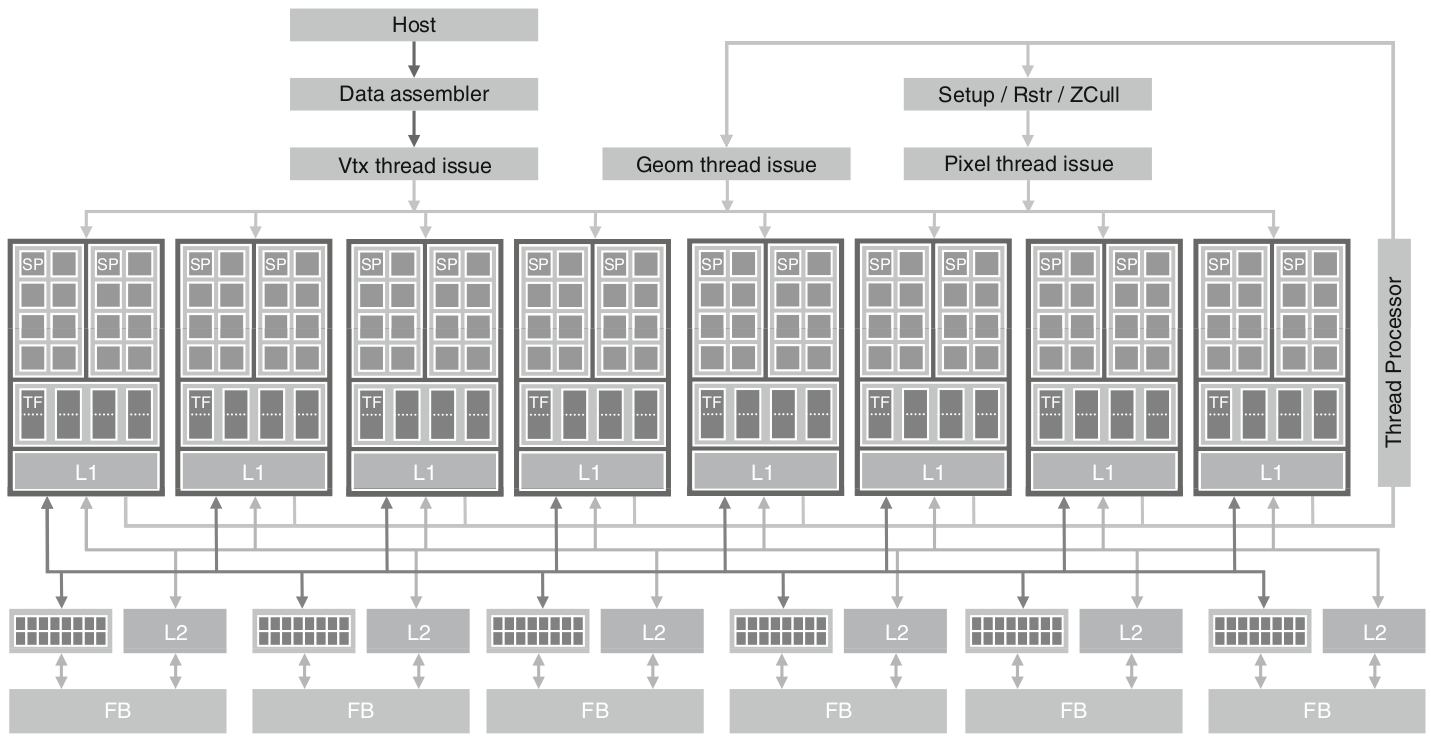
\includegraphics[width=\linewidth]{figs/unified_programmable_processor_array_of_the_GeForce_8800_GTX_graphics_pipeline}
\caption{Unified programmable processor array of the GeForce 8800 GTX}
\label{fig:unified_programmable_processor_array_of_the_GeForce_8800_GTX_graphics_pipeline}
\end{figure}

\section*{The GPGPU Era}
GPU hardware designs evolved towards more unified processors, and were getting
more similar to high-performance parallel computers.
Computations performed by programmable shaders mostly involved matrix and vector
operations, for which GPUs were very well suited (processing blocks of data in
parallel).
The availability of high speed linear algebraic operations, as well as the
unified procesors pushed scientists to start studying the use of GPUs for non-
graphical calculations.
This was achieved through the use of GPGPU techniques.

GPGPU, a shorthand for General Purpose computing on Graphics Processing Units,
consists of using a GPU, which typically only handles computations related to
computer graphics, to perform computations for applications which are
traditionally handled by a CPU.
Such a consideration is possible since GPUs support a functionally complete set
of operations on arbitrary bits, thus can computer any value.

At the time, programmers could only interface with GPUs through graphics APIs
such as the OpenGL or DirectX.
However, APIs had been designed to only match features required in graphics.
To access the computational resources, programmers had to map their problem into
graphics operations so the computations could be launched through OpenGL or
DirectX API calls.
With this consideration in mind, programmers had to arrange their data in such a
way to ``trick'' the GPU in performing the calculations defined in the
programmers' shaders as if they were graphics calculations, whereas in reality,
they were scientific computations.

\subsection*{GPGPU concepts}
There are 4 main GPGPU concepts.

\begin{enumerate}
\item Data arrays are equivalent to GPU textures.
\end{enumerate}

The native data layout for CPUs is the one-dimensional array.

Higher dimensional arrays are available for programmer convenience, but are
actually implemented as one-dimensional arrays, and compilers use linear
transformations to adapt the indices accordingly.

On the other hand, GPUs use two-dimensional arrays as their native data layout,
and are in fact textures.

To make a data array available to the GPU, the CPU would need to create the
data, then map it to a GPU texture which a shader could later read in order to
process.

In order to correctly use the memory available to a GPU, one needs to find a
mapping between the CPU array indices, and the GPU texture coordinates.

Once the mapping is done, the CPU would then transfer the data towards the GPU
texture.

The second GPGPU concept is that computation code (kernel) is equivalent to a
shader.

There is a fundamental difference between the computing model of a CPU and a
GPU, and this impacts the way one needs to think algorithmically.

GPUs follow the data-parallel programming paradigm, whereas CPUs follow the
sequential programming paradigm.

As such, CPUs code is usually implemented as loop-oriented programs, since they
have to iterate over all elements and apply a function to each one.

In contrast, GPUs have highly parallel structures which can apply the same
algorithm to large blocks of data parallely, assuming that there is no
dependence between the operations.

To show the contrast in the programming model, let's compare how one would
compute the addition of 2 N-element vectors and store the result in the first
vector.

Assume we have the following 2 vectors already pre-filled with their respective
data:

int a[N];
int b[N];

The CPU code to perform this vector addition would look like this:

for (int i = 0; i < N; i += 1)
{
    a[i] = a[i] + b[i];
}

Note that the CPU will have to loop over all indices of the 2 arrays, and add
each element one by one in a sequential way.

It is important to note that each of the N computations are completely
independent, as for a given output index, there are distinct input memory
locations, and there are no data dependencies between elements in the result
vector.

For example, once we have computed a[0] = a[0] + b[0], its result will be of no
help when it comes to computing a[1] = a[1] + b[1].

As such, assuming we have a computation unit with N parallel structures, we
would be able to compute the vector addition without the need of any loop by
assigning one vector element addition to each computation element.

This is easily done by adapting the index of the vector elements that are
provided to each computation unit.

This is the core idea behind GPGPU computing: separating the identical, but
independent calculations from one another, and assigning them to execution units
which can then execute them at the same time.

Algorithms are extracted into computational kernels which are no longer vector
expressions, but scalar templates of the algorithm that form a single output
value from a set of input values.

These algorithms are implemented in shaders which will then calculate the
independent computations parallely.

For the vector addition used above, the 2 vectors will have to be written into
textures by the CPU, then the shader will read the appropriate elements from the
texture to perform its independent computation.

The third GPGPU concept is that computations are equivalent to "drawing".

Indeed, the final output of a GPU is an "image", therefore all computations have
to, in some way or another, write their "results" to the frame buffer for it to
be available to the programmer.

Therefore, the programmer must tell the graphics API (either OpenGL or DirectX)
to draw a rectangle over the whole screen (since our screens are rectangles), so
that the fragment shader can apply its code to each pixel independently and
output an answer.

If the API were not instructed to draw something that fills the whole screen,
then the fragment shader's code would not be applied to all our data in the
textures we created, but only to a subset of it.

By rendering the simple rectangle, we can be sure that the kernel is executed
for each data item in the original texture.

The fourth GPGPU concept is feedback.

On CPUs, data is read from memory locations, and results are written to memory
locations.

On GPUs, we just saw that the final output is written to the frame buffer.

However, a huge number of algorithms are not straight-line code, and require the
GPU's result to be used as input for another subsequent computation.

To achieve this on a GPU, we need to execute another rendering pass

This is achieved by writing the current result to another texture, binding this
texture as well as another input and output textures, and potentially also
binding another shader for the algorithm to continue.

This is known as the ping-pong technique since one has to keep juggling between
textures until the algorithm is done and the result is outputted to the frame
buffer.

To recap all that is needed for GPGPU on graphics APIs, one needs to create data
on the CPU, map it to GPU textures, write shaders to perform computations based
on the data in the textures, and finally write the result back to the frame
buffer.

As one can see, early GPGPU programming can quickly become quite tedious, even
for simple algorithms, as one must understand the complete graphics rendering
pipeline in order to trick the GPU in thinking it's performing graphics
calculations, whereas the programmers are actually manipulating their data on
GPU textures, and writing their kernels in shaders.

Indeed, graphics APIs were not intended for scientific computations, and are
thus not easily programmable.

In order to fully benefit from the parallel processing power of GPUs without
having to know anything about the graphics rendering pipeline, more
computational oriented languages were created.

% Nvidia CUDA:
% ------------
% The Compute Unified Device Architecture, more commonly known under the name
% CUDA, is a parallel computing platform and programming model developed by
% NVIDIA in 2006, and implemented by the GPUs they produce.

% CUDA was designed for GPGPU programming, as developers can compile C code for
% CUDA capable GPUs, thus avoiding the tedious work of mapping their algorithms to
% graphics concepts.

% Essentially, CUDA's main advantage is that developers have explicit access to
% the GPUs virtual instruction, as well as its device memory.

% By using CUDA, developers can use GPUs in a similar way as CPUs, without having
% to know anything about the graphics rendering pipeline.

% CUDA also exposes several GPU hardware features that are not accessible through
% graphics APIs, the most important of which is access to GPU shared memory, an
% area of on-chip GPU memory which can be accessed in parallel by several blocks
% of threads.

% CUDA also supports a thread synchronization primitive, allowing cooperative
% parallel processing of on-chip data, greatly reducing the high-latency off-chip
% bandwidth requirements of many parallel algorithms.

% CUDA Program Structure:
% -----------------------
% A CUDA program consists of multiple interleavings of CPU (host) code segments,
% and GPU (device) code segments.

% The segments that exhibit little data parallelism are implemented as host code,
% whereas the data parallel segments are implemented as device code.

% < insert graphics: execution of cuda program >

% All the code is written in ANSI C extended with keywords for labeling data-
% parallel functions called kernels, and their associated data structures.

% The compilation process separates the host code from the device code, passing
% the host code to the host's standard C compiler, and the device code to the
% NVIDIA C compiler (nvcc).

% In CUDA, computations are carried out by threads, a large number of which are
% generated by kernels to exploit data parallelism.

% Kernels specify the code to be executed by all threads during a parallel
% segment.

% All the threads execute the same code, thus CUDA programming follows the SIMT
% (Single Instruction Multiple Thread) programming style.

% CUDA Thread Organization:
% -------------------------
% When a kernel is launched, a grid of parallel threads are executed.

% Threads in a grid are organized into a two-level hierarchy, as shown in the
% figure below.

% < insert graphics: cuda thread organization >

% A grid consists of one or more thread blocks, each of which contain the same
% number of threads.

% Each thread block has a unique 1D, 2D, or 3D block identifier (note that for
% simplicity, a 2D identifier is drawn in the figure above).

% Similarly, each thread within a block has a unique 1D, 2D, or 3D thread
% identifier.

% With NVIDIA's Fermi (compute capability 2.0) and Kepler (compute capability 3.0)
% architectures, a maximum of 1024 threads can be contained in a block.

% Once a kernel is launched, the CUDA runtime generates the corresponding grid of
% threads, which are then assigned to execution resources on a block-by-block
% basis.

% CUDA execution resources are organized into streaming multiprocessors (SMs), two
% of which are shown in the following figure.

% < insert graphics: thread block assignment to SMs >

% A maximum number of blocks can be assigned to each SM (8 on Fermi GPUs, and 16
% on Kepler GPUs) as long as there are enough resources to satisfy the needs of
% all the blocks.

% If any of the resources needed for the simultaneous execution of the blocks are
% unavailable, less blocks will be scheduled for execution on the SM.

% The remaining blocks will execute once the resources needed are available again.

% Although blocks are scheduled to be run on an SM, it is the threads of that
% block that execute the computations.

% All threads of a block are scheduled for execution in structures called warps,
% each of which contain 32 continuous threads (identified by their threadIdx
% values).

% A crucial aspect about warps is that the hardware executes an instruction for
% all threads in the same warp before moving to the next instruction.

% It works well when all threads within a warp follow te same control flow path
% when working on their data.

% For example, branch statements work well when either all threads take the then
% statement, or all the threads take the else statement.

% If some threads execute the then part, and others execute the else part, the
% SIMT execution no longer works and the warps execution will require multiple
% passes through the divergent paths.

% One pass will be needed for each divergent path.

% These passes occur sequentially, thus increasing the execution time.

% The situation is even worse for loops, therefore it is very important to try and
% keep thread divergence low.

% CUDA Memory Structure:
% ----------------------
% In CUDA, the host and devices have separate memory spaces, as GPUs are typically
% hardware cards that come with their own DRAM.

% In order to provide data to a kernel, memory needs to be allocated on the
% device, and data has to be transferred to the allocated memory.

% Similarly, after kernel completion, device results must be transferred back from
% device memory to host memory.

% CUDA devices have several different memory types available to developers.

% < insert graphics: cuda memory hierarchy >

% Note that texture memory is not shown in the above figure.

% At the bottom of the figure, we see global memory, and constant memory, the 2
% off-chip memories available on a CUDA GPU.

% Global memory is memory to which the host can write data to, and read data from.

% Global memory is typically implemented as DRAM, and suffers from long access
% latencies, and finite access bandwidth.

% Constant memory supports short-latency, high-bandwidth, read-only access by the
% device when all threads simultaneously access the same location.

% Registers and shared memory are on-chip memories, and are thus accessible at
% very high speeds, and in a parallel way.

% Global Memory Coalescing:
% -------------------------
% Because of the high access latencies of DRAM, global memory is organized in such
% a way that when reading a certain location, several consecutive memory locations
% are returned.

% If an application can make use of multiple consecutive global memory locations
% before moving to other locations, the DRAMs can supply the data at a much higher
% rate than if random locations are accessed.

% When all threads in a warp execute a load instruction, the hardware detects
% if the threads access consecutive global memory locations.

% If it is the case, then it does not issue multiple load instruction, but will
% combine, or coalesce them into less read instructions.

% Therefore, to achieve anywhere close to the peak advertised global memory
% bandwidth, it is important to take advantage of memory coalescing, by organizing
% data in memory in such a way that each thread can read the data it needs at the
% same time as the other threads.

% Lets demonstrate this on an example where threads try to read a matrix.

% For example, normal CPU C code for accessing a 4x4 matrix would ressemble the
% following:

% int matrix[4][4];

% < insert graphics: 4x4 matrix drawing >

% for (int i = 0; i < 4; i++)
% {
%     for (int j = 0; j < 4; j++)
%     {
%         matrix[i][j] = ... ;
%     }
% }

% If we use 4 GPU threads, we get the following code:

% for (int j = 0; j < 4; j++)
% {
%     matrix[threadIdx.x][j] = ... ;
% }

% This matrix is stored in memory as a continuous 1D array of data, and accessing
% the data on the GPU with 4 threads parallely would look like this (1st loop
% iteration):

% < insert graphics: 1D 16-element drawing with arrows every 4 blocks >

% Note that each thread tries to load its "line" at the same time as the others.

% This results in 4 scattered global memory reads.

% What we would want to have, is reads of the following form:

% < insert graphics: 1D 16-element drawing with arrows on the first 4 blocks >

% The code corresponding the the above memory access pattern is:

% for (int j = 0; j < 4; j++)
% {
%     matrix[j][threadIdx.x] = ... ;
% }

% But then, each thread would no longer be accessing the element it initially
% wanted.

% The solution to this problem is to transpose the initial matrix, thus yielding
% the following 1D memory access pattern:

% < insert graphics: transposed matrix >

% < insert graphics: 1D matrix, but with 4 arrows on first 4 blocks, and indices
% correct this time (transposed) >

% This yields perfect coalescing, resulting in minimal global memory accesses.

% Therefore, a "simple" port from C code is to transpose arrays, since they are
% mostly accessed one row at a time, whereas GPUs can load one column at a time
% better for each thread's data to be fetched at the same time.

% One must strive for perfect coalescing per warp by aligning starting addresses
% (may need padding), and accessing continuous memory regions.

% General performance considerations summary:
% -------------------------------------------
% So, in order to maximize the use of all execution units on a CUDA GPU, it is
% important to make sure global memory reads and writes are coalesced whenever
% possible.

% If memory coalescing is not done, then all other "optimizations" would not be
% very significant.

% In case they are difficult to coalesce, it is better to try and use 1D texture
% lookups instead.

% One should make use of shared memory as much as possible, as it is much faster
% than global memory.

% If possible, avoid divergent branches at all cost, otherwise, keep them low.
%
% --------------------------------------------------------------------------------
% Bibliography:
% -------------
% Internet:
% ---------
% http://en.wikipedia.org/wiki/Graphics_processing_unit
% http://en.wikipedia.org/wiki/Programmable_shader
% http://en.wikipedia.org/wiki/General-purpose_computing_on_graphics_processing_units
% http://en.wikipedia.org/wiki/Functional_completeness
% http://www.mathematik.uni-dortmund.de/~goeddeke/gpgpu/tutorial.html
% http://en.wikipedia.org/wiki/CUDA
% https://developer.nvidia.com/cuda-faq
% https://developer.nvidia.com/get-started-cuda-cc
%
% Books:
% ------
%
% Papers:
% -------


\end{document}
